% !TEX root = MATLAB_Introduction_Blair.tex

% ============================================
% ============================================
\section{Basic Visualization}
The code of Example \ref{Exmp:Cosines} executes, but we have not yet shown a way to visualize the result to verify the calculation. To do this, we introduce basic plotting.

A very useful command is the \texttt{plot()} command, which can make line graphs. One very general syntax for \texttt{plot()} is of the form \verb!plot(X1, Y1, X2,Y2, X3, Y3,...)!, where \texttt{Xk} and \texttt{Yk} are vectors of equal length storing $x$-data and $y$-data, respectively, with $k \in \{1, 2, 3, \ldots\}$. To adapt this syntax to the code of Example \ref{Exmp:Cosines}, we use \texttt{t} in the place of each of \texttt{X1}, \texttt{X2}, \texttt{X3}, and \texttt{X4}. Also, we use \texttt{fn(:,}$k$\texttt{)} in place of \verb!Y!$k$.
% vvv------------------------------------------------------------vvv
\begin{lstlisting}[style=Matlab-editor]
plot( t, fn(:,1), t, fn(:,2), t, fn(:,3), t, fn(:,4) );
\end{lstlisting}
% ^^^------------------------------------------------------------^^^

In the case of Example \ref{Exmp:Cosines}, however, \texttt{X1}, \texttt{X2}, \texttt{X3}, and \texttt{X4} are indentically equal to the \texttt{t} vector; additionally, all the sets of $y$-data are stored as rows of the \texttt{fn} matrix. In this case, we can use the simpler syntax
% vvv------------------------------------------------------------vvv
\begin{lstlisting}[style=Matlab-editor]
plot( t, fn);
\end{lstlisting}
% ^^^------------------------------------------------------------^^^
The result of this listing or the prior one are equivalent. We append this visualization code to the end of \texttt{Sinusoids.m}, resulting in a new script, \verb!Sinusoids_v01.m!:
% vvv------------------------------------------------------------vvv
\begin{lstlisting}[style=Matlab-editor]
% Sinusoids_v01.m
% 
% This is the same as Sinusoids.m, but adds visualization.
%
% By E.P. Blair
% Baylor University
%

nt = 75; % number of time points
t = linspace(0, 1, nt); % [s] define a time vector

fn = zeros(4, nt); % Define a storage array to hold fn calculations
                   % The n^th row of fn stores fn = cos(2*pi*n*t)
      
% calculate fn and store fn for each value of n in the n^th row
fn(1,:) = cos(2*pi*t); % n = 1
fn(2,:) = cos(2*pi*2*t); % n = 2
fn(3,:) = cos(2*pi*3*t); % n = 3
fn(4,:) = cos(2*pi*4*t); % n = 4

plot(t, fn);
\end{lstlisting}
% ^^^------------------------------------------------------------^^^
The result of this listing is shown in Fig.\ \ref{fig:Sinusoids_v01}. Here, we see the set of sinusoids represented by $f_n (t)$ plotted for $n \in \{1, 2, 3, 4\}$. However, this plot may be improved in several ways:
\begin{enumerate}
\item The sinusoids are not smooth: they look as though they are only approximated using straight line segments. plot requires labels that help assign meaning to the data.
\item This plot requires labels that help assign meaning to the data.
\begin{enumerate}
\item The $x$-axis and $y$-axis both need \textit{labels}.
\item There should be a \textit{legend} to disambiguate the various lines in the plot.
\end{enumerate}

\item A grid may be added to assist in reading the graph.
\item The data lines themselves may be thickened for improved visibility.
\end{enumerate}

These changes can be achieved by using \verb!Sinusoids_v02.m!:
% vvv------------------------------------------------------------vvv
\begin{lstlisting}[style=Matlab-editor,label=lstSinusoids_v02, caption={Listing of the \texttt{Sinusoids\_v02.m} script.}]
% Sinusoids_v02.m
% 
% This is the same as Sinusoids_v01.m, but improves the visualization.
%
% By E.P. Blair
% Baylor University
%

nt = 150; % number of time points
t = linspace(0, 1, nt); % [s] define a time vector

fn = zeros(4, nt); % Define a storage array to hold fn calculations
                   % The n^th row of fn stores fn = cos(2*pi*n*t)
      
% calculate fn and store fn for each value of n in the n^th row
fn(1,:) = cos(2*pi*t); % n = 1
fn(2,:) = cos(2*pi*2*t); % n = 2
fn(3,:) = cos(2*pi*3*t); % n = 3
fn(4,:) = cos(2*pi*4*t); % n = 4

plot(t, fn, 'LineWidth', 2); % thickens the data lines
grid on; % makes the grid visible
set(gca, 'FontSize', 18, 'FontName', 'Times');
xlabel('$t$ (s)', 'Interpreter', 'latex')
ylabel('$f_n(t)$', 'Interpreter', 'latex')
sine_lgnd = legend('$f_1$', '$f_2$', '$f_3$', '$f_4$')
sine_lgnd.Interpreter = 'latex';
\end{lstlisting}
% ^^^------------------------------------------------------------^^^
In this listing, line 9 increases the number of data points so that the plots become smoother. Line 21 uses optional inputs to \verb!plot()! in a \textbf{property-value} pair, specifically, \verb!`LineWidth', 2! to increase the weight of the lines drawn. Line 22 turns the grid on. Line 23 uses \texttt{gca} (get current axes) to get a handle to the current axes. This handle, then is used within the \texttt{set()} function to modify properties of the current axes using property-value pairs. Specifically, we set the font size to 18, and the font name to \texttt{'Times'}. Lines 24 and 25 generate the labels for the $x$- and $y$-axes. Notice here that the first argument to \texttt{xlabel()} or \texttt{ylabel()} is the desired string, and that some of the string is enclosed in dollar signs (\verb!$!). These tell MATLAB to use \LaTeX \, syntax to mathematically typeset the expression or equation contained inside the paired \verb!$! signs. In order for this to work, we can to use the property value pair \verb!'Interpreter', 'latex'! to indicate that MATLAB needs to perform some \LaTeX \, typesetting. In line 26, we use the \texttt{legend()} command to create the legend, and we save the handle by which we reference the legend object by assigning it to a variable, \verb!sine_lgnd!. The inputs to \texttt{legend()} are character strings, and again, we used \LaTeX \, formatting. In order for this to work, we set the \texttt{Interpreter} property of \verb!sine_lgnd!  to \verb!'latex'!. The result of this code is shown in Fig.\ \ref{fig:Sinusoids_v02}.

\begin{figure}[htbp] %  figure placement: here, top, bottom, or page
   \centering
   \subfigure[Output for listing of \texttt{Sinusoids\_v01.m}.]{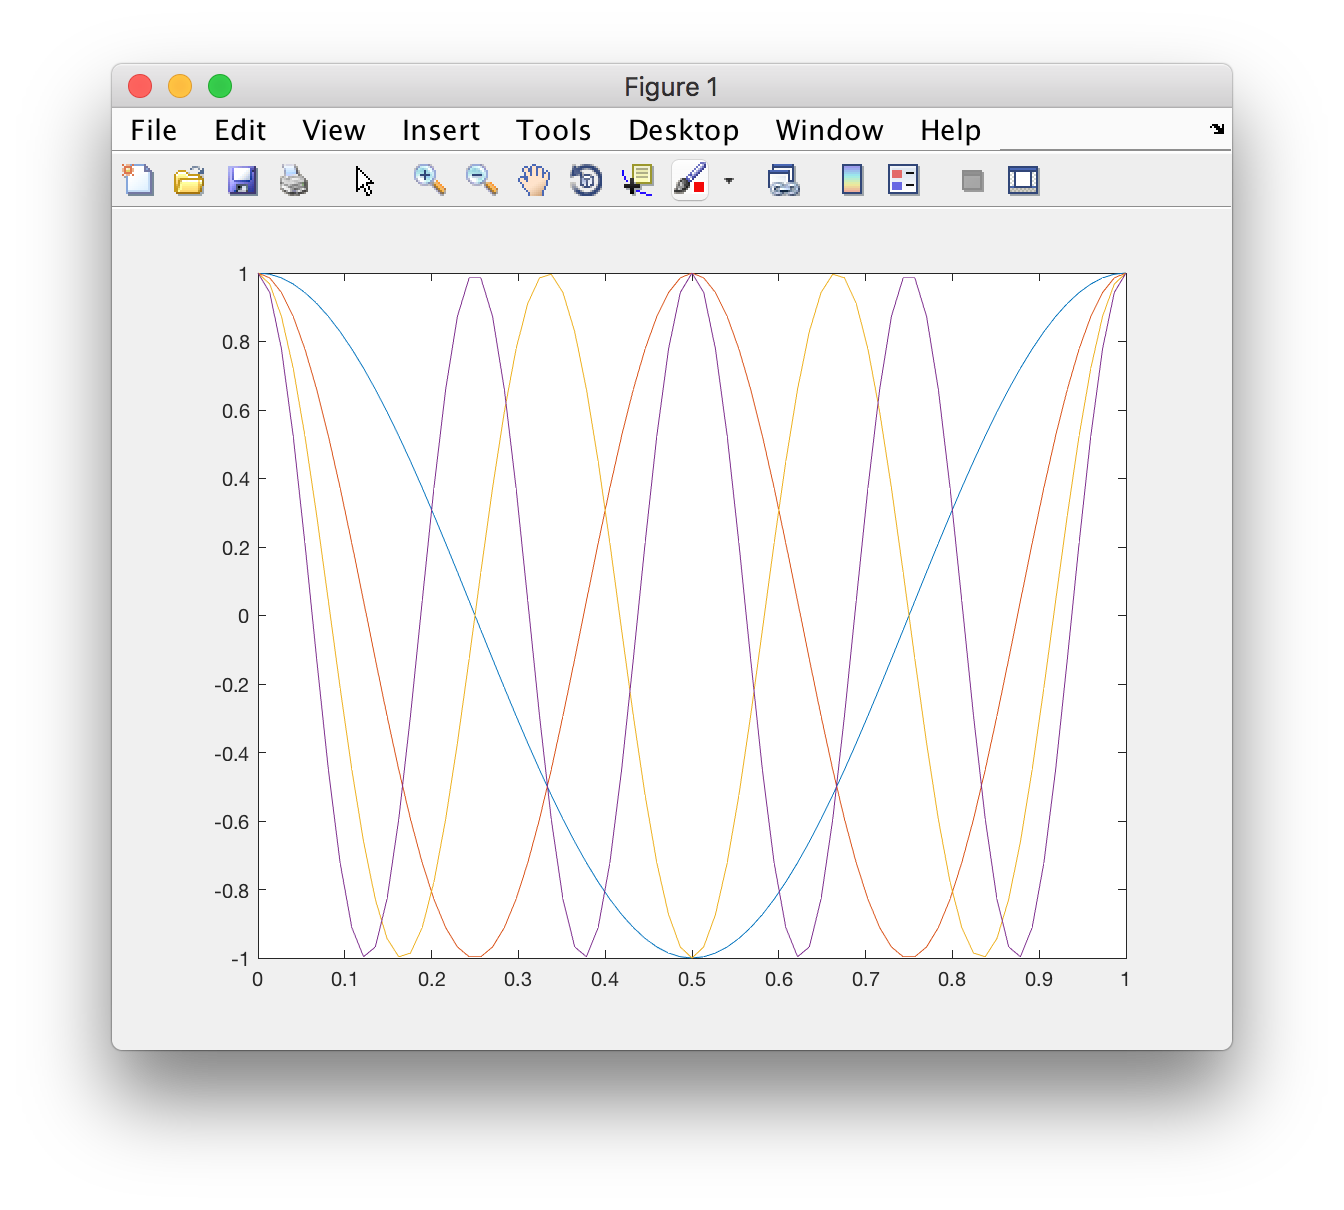
\includegraphics[width=0.485\textwidth]{graphics/Fig_Sinusoids_v01.png} \label{fig:Sinusoids_v01}
   }
   \subfigure[Output for listing of \texttt{Sinusoids\_v02.m}.]{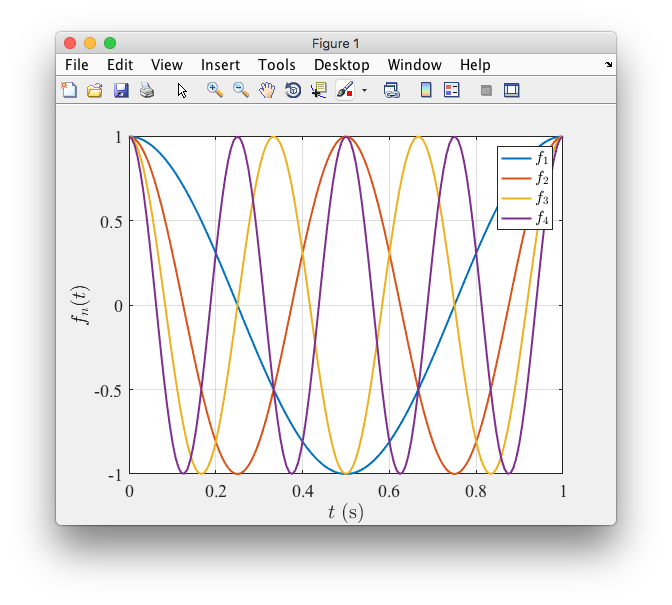
\includegraphics[width=0.485\textwidth]{graphics/Fig_Sinusoids_v02.png} \label{fig:Sinusoids_v02}
   }
   \caption{Plots of the sinusoids calculated in Example \ref{Exmp:Cosines}.}
   \label{fig:Sinusoids_output}
\end{figure}
